\begin{figure*}[htbp]
    \centering
    \begin{tabular}{m{50mm} m{50mm} m{50mm} m{10mm}}
        % first row
        \begin{minipage}[b]{\linewidth}
            \centering
            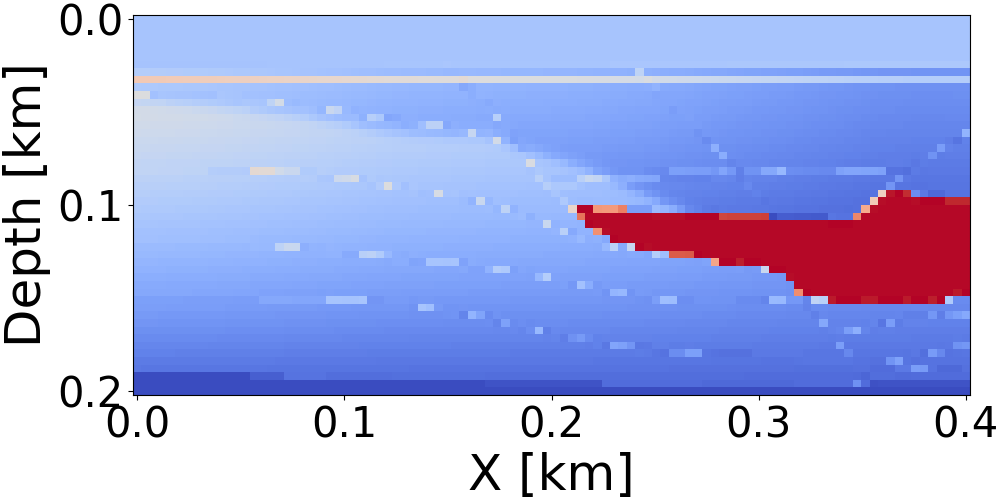
\includegraphics[width=\linewidth]{public/true}
            \vspace{-9mm}
            \caption*{\raisebox{-2mm}{\footnotesize Ground truth}}
            \vspace{1mm}
        \end{minipage} &
        \begin{minipage}[b]{\linewidth}
            \centering
            
\includegraphics[width=\linewidth]{public/initial}
            \vspace{-9mm}
            \caption*{\raisebox{-2mm}{\footnotesize Initial model}}
            \vspace{1mm}
        \end{minipage} &
        \begin{minipage}[b]{\linewidth}
            \centering
            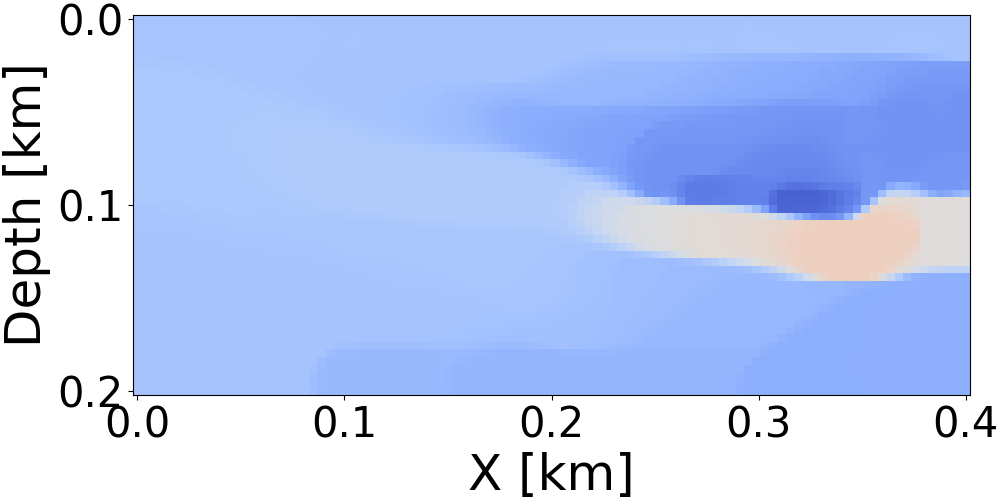
\includegraphics[width=\linewidth]{public/alpha_150}
            \vspace{-7mm}
            \caption*{\footnotesize Proposed Method, $\alpha = 150$}
            \vspace{1mm}
        \end{minipage} &
        \multirow[t]{3}{*}{\raisebox{-66mm}{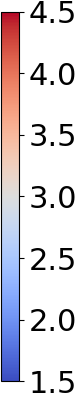
\includegraphics[height=50mm]{public/color-bar}}} \\

        % second row
        \begin{minipage}[b]{\linewidth}
            \centering
            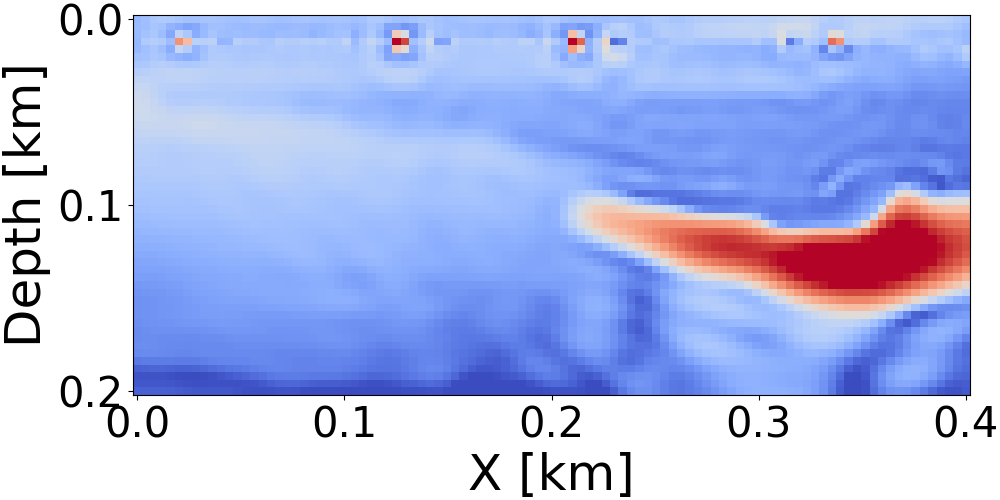
\includegraphics[width=\linewidth]{public/gradient}
            \vspace{-9mm}
            \caption*{\raisebox{-2mm}{\footnotesize The Standard FWI Method}}
            \vspace{1mm}
        \end{minipage} &
        \begin{minipage}[b]{\linewidth}
            \centering
            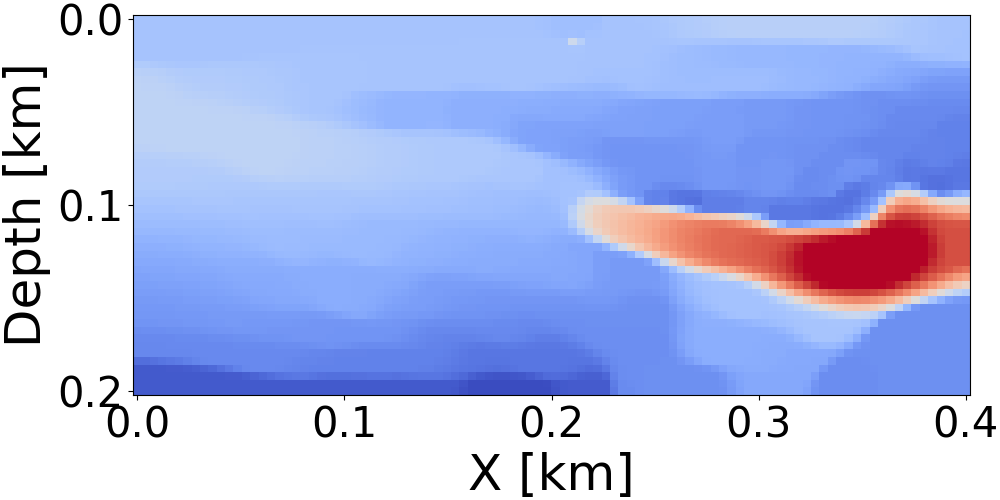
\includegraphics[width=\linewidth]{public/alpha_350}
            \vspace{-7mm}
            \caption*{\footnotesize Proposed Method, $\alpha = 350$}
            \vspace{1mm}
        \end{minipage} &
        \begin{minipage}[b]{\linewidth}
            \centering
            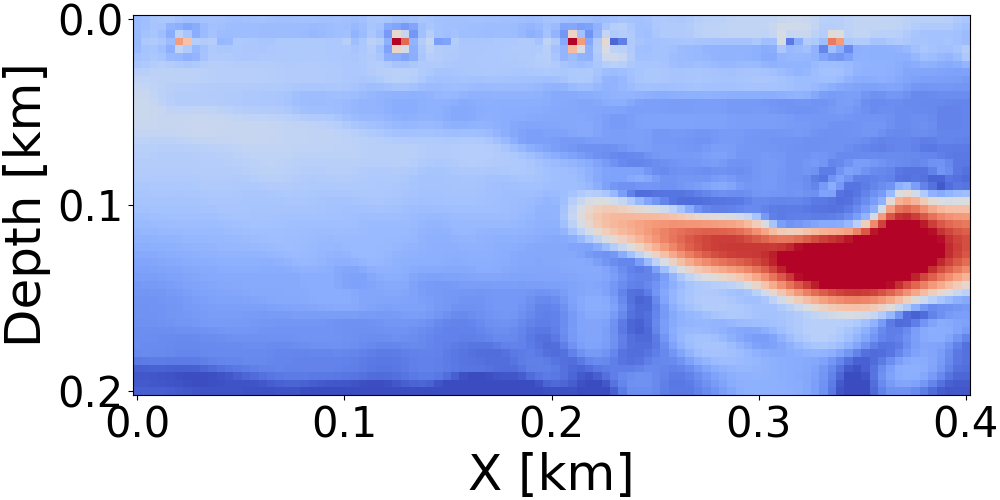
\includegraphics[width=\linewidth]{public/alpha_550}
            \vspace{-7mm}
            \caption*{\footnotesize Proposed Method, $\alpha = 550$}
            \vspace{1mm}
        \end{minipage} \\

        % third row
        \begin{minipage}[b]{\linewidth}
            \centering
            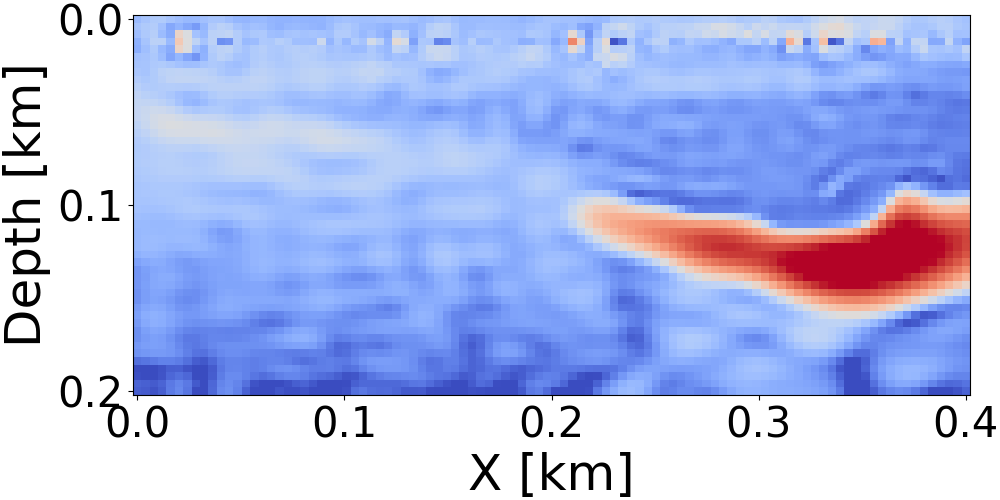
\includegraphics[width=\linewidth]{public/gradient_noisy}
            \vspace{-7mm}
            \caption*{\footnotesize The Standard FWI Method \\ (with the noisy observed seismic data)}
            \vspace{1mm}
        \end{minipage} &
        \begin{minipage}[b]{\linewidth}
            \centering
            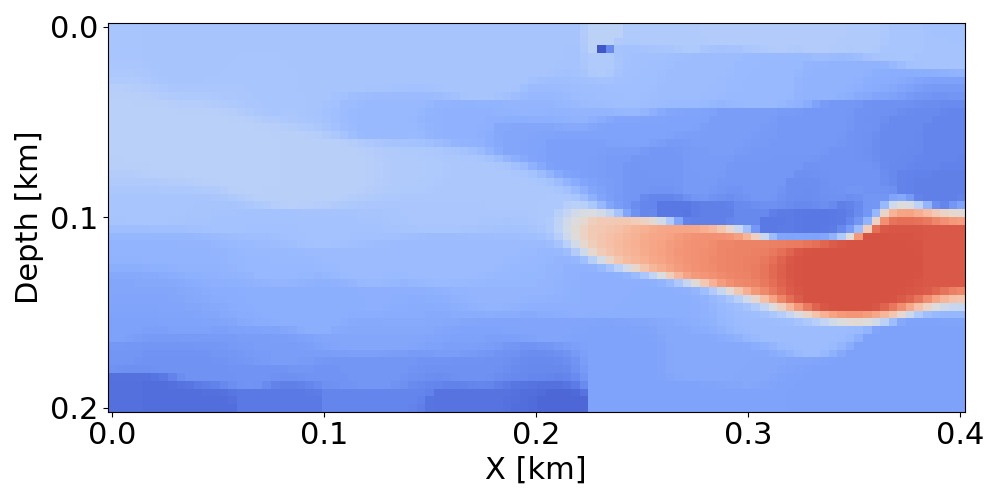
\includegraphics[width=\linewidth]{public/alpha_300_noisy}
            \vspace{-7mm}
            \caption*{\footnotesize Proposed Method, $\alpha = 300$ \\ (with the noisy observed seismic data)}
            \vspace{1mm}
        \end{minipage} &
    \end{tabular}
    \vspace{-3mm}
    \caption{Velocity models [km/s] and their corresponding reconstructions.}
    \label{fig:velocity-models}
\end{figure*}
